\section{Data Sanitization}
	
In diesem Kapitel wird näher auf den Programmcode des vorliegenden Forschungsprojektes eingegangen und erklärt, was genau in der Datensammlung und Datenverarbeitung gemacht wurde. Zu Beginn wurden die Daten wie in Punkt \textit{2.1.1 GetOldTweets3} beschrieben, mit der Bibliothek gescrapt und als CSV-Datei abgespeichert. Wie das Scraping in der Bibliothek genau funktioniert, ist ebenfalls unter dem Punkt \textit{2.1.1. GetOldTweets3} beschrieben. Um die gespeicherten Tweets für das MapReduce vor zu verarbeiten, wurden die zur Verfügung stehenden Bibliotheken \textit{NLTK} und \textit{cleantext}.
	
	
	\begin{figure}[ht]
		\centering
		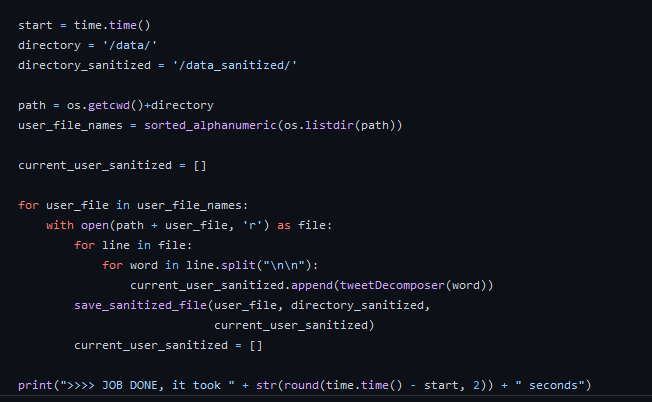
\includegraphics[width=0.9\textwidth]{images/Kapitel2/Code_Datensanierung_1}
		\caption{\label{fig:DataSan}Sanierungs-For-Schleife der Daten}
	\end{figure}
	
Die Variable "directory" und "directory\_ sanitized" geben den Pfad an, in welchem Ordner die Daten gespeichert werden sollen. Mit der Bibliothek \textit{os} von Python können über "os.listdir(pfad)" alle Dateinamen innerhalb dieses Ordners eingelesen werden. Mit der Variable "user\_ file\_ names" wird eine alphanumerisch sortierte Liste der Usernamen der Politiker zurückgegeben, welche dann über eine For-Schleife durchgegangen werden kann, da der Name der CSV-Dateien mit folgendem Muster dem Usernamen entspricht, "Name\_ D" oder "Name\_ R". \textbf{D} steht für demokratisch und \textbf{R} für republikanisch. In dieser Datensanierungsschleife wird die Funktion \textit{tweetDecomposer} verwendet. Diese Funktion übernimmt in der vorliegenden Datensanierung die Hauptaufgabe.
	
%	\begin{figure}[ht]
%		\centering
%		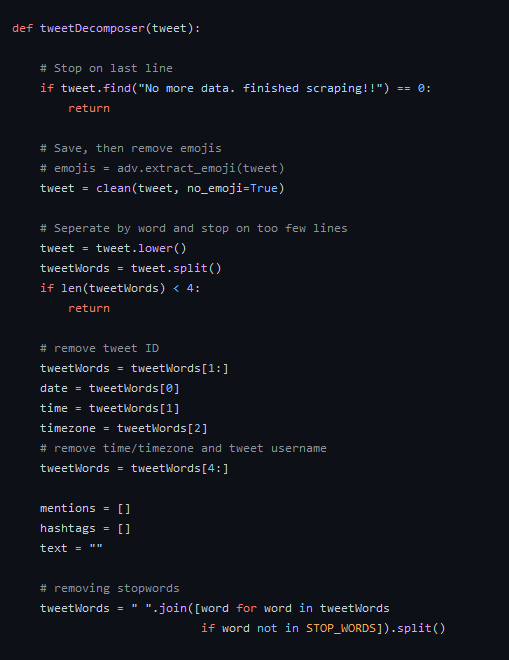
\includegraphics[width=0.9\textwidth]{images/Kapitel2/Code_Datensanierung_2}
%		\caption{\label{fig:DataSanF1}Ausschnitt eins der Sanierungsfunktion der Daten}
%	\end{figure}

Mit der Bibliothek \textit{cleantext} wurden \textit{Emojis} aus dem Text entfernt, wie man in Abbildung ~\ref{fig:DataSanF1} in den ersten Zeilen der Funktion sehen kann. Dann werden alle Worte innerhalb eines Tweets kleingeschrieben und aufgetrennt, damit die ID, die Zeitzone und der Username aus dem Tweet entfernt werden können. Mit \textit{NLTK} werden dann die Stoppworte durch ein \textit{join} aus den Tweets entfernt, sodass man zu den letzten Datensanierungsschritten kommen kann.
	 
%	\begin{figure}[ht]
%		\centering
%		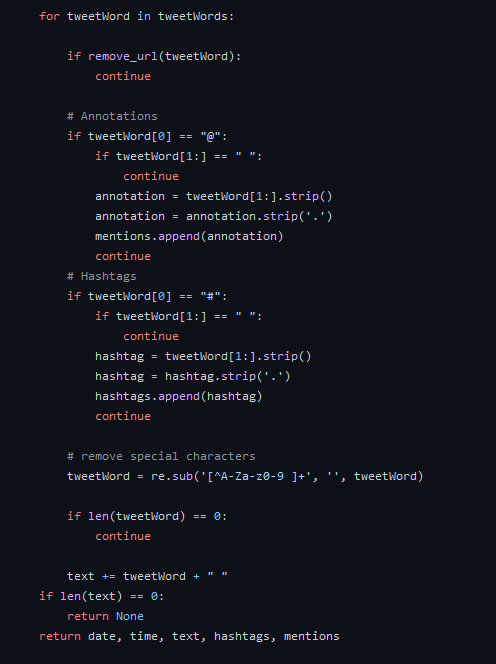
\includegraphics[width=0.9\textwidth]{images/Kapitel2/Code_Datensanierung_3}
%		\caption{\label{fig:DataSanF1}Ausschnitt eins der Sanierungsfunktion der Daten}
%	\end{figure}
	
Da die Annotations und Hashtags gespeichert werden sollen, wurde, wie in Abbildung ~\ref{fig:DataSanF2} zu sehen ist, eine extra For-Schleife eingesetzt. Die For-Schleife läuft über den gesamten Input des Tweets, dazu zählen Datum, Zeit, Username, Hashtag und Emoji. Als Erstes wird überprüft, ob es sich um eine URL handelt oder nicht. Tritt der Fall ein, dass es eine URL ist, wird diese einfach übersprungen und nicht mit abgespeichert. Die Annotations können durch ein "@" erkannt werden, während die Hashtags mit einem "\# " erkannt werden. Beide Erkennungsmarker werden nicht mit abgespeichert. Der restliche Inhalt des Hastags und der Annotation werden in einer extra Liste gespeichert.


Als Letztes wurden alle Sonderzeichen wie Punkte, Kommas und andere Zeichen entfernt. Die Funktion gibt dann alle interessanten Daten für die Analyse zurück. Zum Schluss werden diese Daten in einer CSV-Datei gespeichert. Als nächster Schritt folgt die Hautanalyse unseres Projektes in 2.3.